% This file was converted to LaTeX by Writer2LaTeX ver. 1.4
% see http://writer2latex.sourceforge.net for more info
\documentclass[a4paper]{article}
\usepackage[latin1]{inputenc}
\usepackage[T1]{fontenc}
\usepackage[english]{babel}
\usepackage{amsmath}
\usepackage{amssymb,amsfonts,textcomp}
\usepackage{color}
\usepackage{array}
\usepackage{supertabular}
\usepackage{hhline}
\usepackage{hyperref}
\hypersetup{pdftex, colorlinks=true, linkcolor=blue, citecolor=blue, filecolor=blue, urlcolor=blue, pdftitle=, pdfauthor=Oscar Daniel, pdfsubject=, pdfkeywords=}
\usepackage[pdftex]{graphicx}
\makeatletter
\newcommand\arraybslash{\let\\\@arraycr}
\makeatother
% Page layout (geometry)
\setlength\voffset{-1in}
\setlength\hoffset{-1in}
\setlength\topmargin{1in}
\setlength\oddsidemargin{1in}
\setlength\textheight{9.6929in}
\setlength\textwidth{6.2681in}
\setlength\footskip{0.0cm}
\setlength\headheight{0cm}
\setlength\headsep{0cm}
% Footnote rule
\setlength{\skip\footins}{0.0469in}
\renewcommand\footnoterule{\vspace*{-0.0071in}\setlength\leftskip{0pt}\setlength\rightskip{0pt plus 1fil}\noindent\textcolor{black}{\rule{0.0\columnwidth}{0.0071in}}\vspace*{0.0398in}}
% Pages styles
\makeatletter
\newcommand\ps@Standard{
  \renewcommand\@oddhead{}
  \renewcommand\@evenhead{}
  \renewcommand\@oddfoot{}
  \renewcommand\@evenfoot{}
  \renewcommand\thepage{\arabic{page}}
}
\makeatother
\pagestyle{Standard}
\setlength\tabcolsep{1mm}
\renewcommand\arraystretch{1.3}
\title{}
\author{Oscar Daniel}
\date{2015-03-19}
\begin{document}
\begin{flushleft}
\tablefirsthead{}
\tablehead{}
\tabletail{}
\tablelasttail{}
\begin{supertabular}{|m{0.5872598in}|m{0.82335985in}|m{0.9476598in}|m{0.8643598in}|m{0.76015985in}|m{2.37956in}|}
\hline
Test number &
Description &
Data Type  &
Expected Result &
Pass/Fail &
Cross Reference\\\hline
1 &
Checking that the login screen allows user to log in with their credentials. &
Typical &
System logs in using the user's data. &
Pass &
 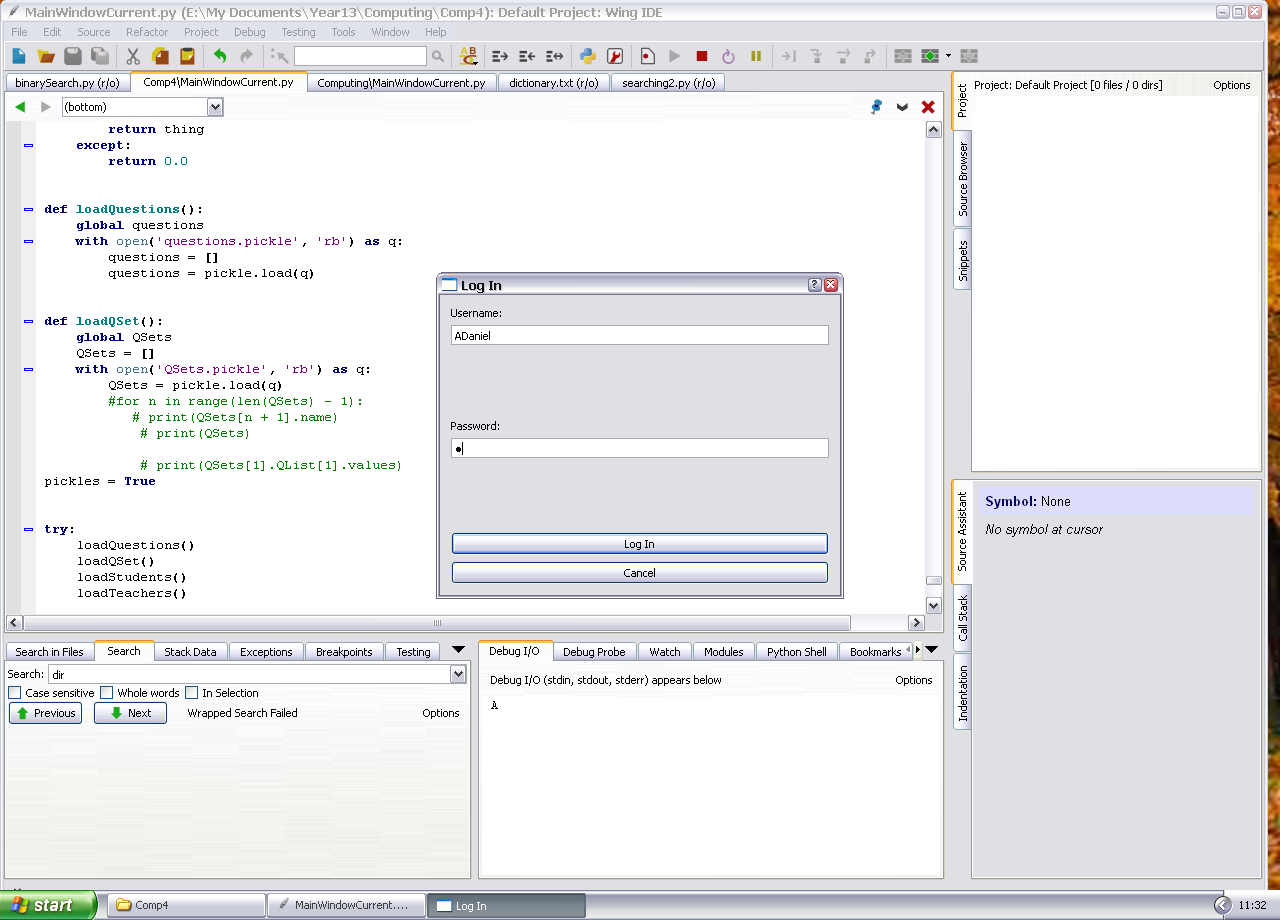
\includegraphics[width=2.0429in,height=1.652in]{TestTable-img001.png} 
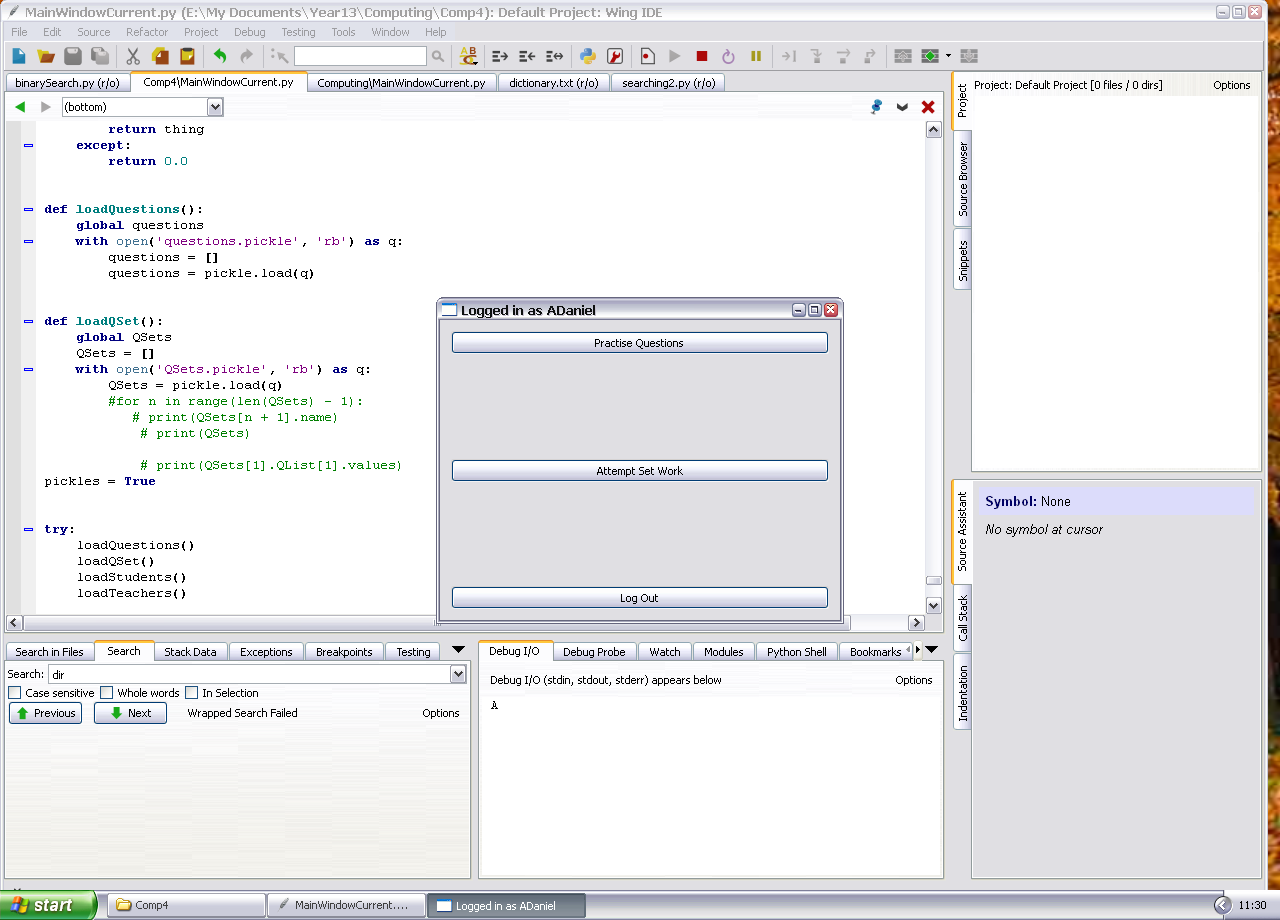
\includegraphics[width=2.0866in,height=1.7217in]{TestTable-img002.png} \\\hline
2 &
Checking that the log in screen does not allow people to log in with any credentials. &
Erroneous.\newline
(Incorrect Password) &
Error message appears.\newline
(Your Username or Password is incorrect. Please try again.) &
Pass &
~

~

 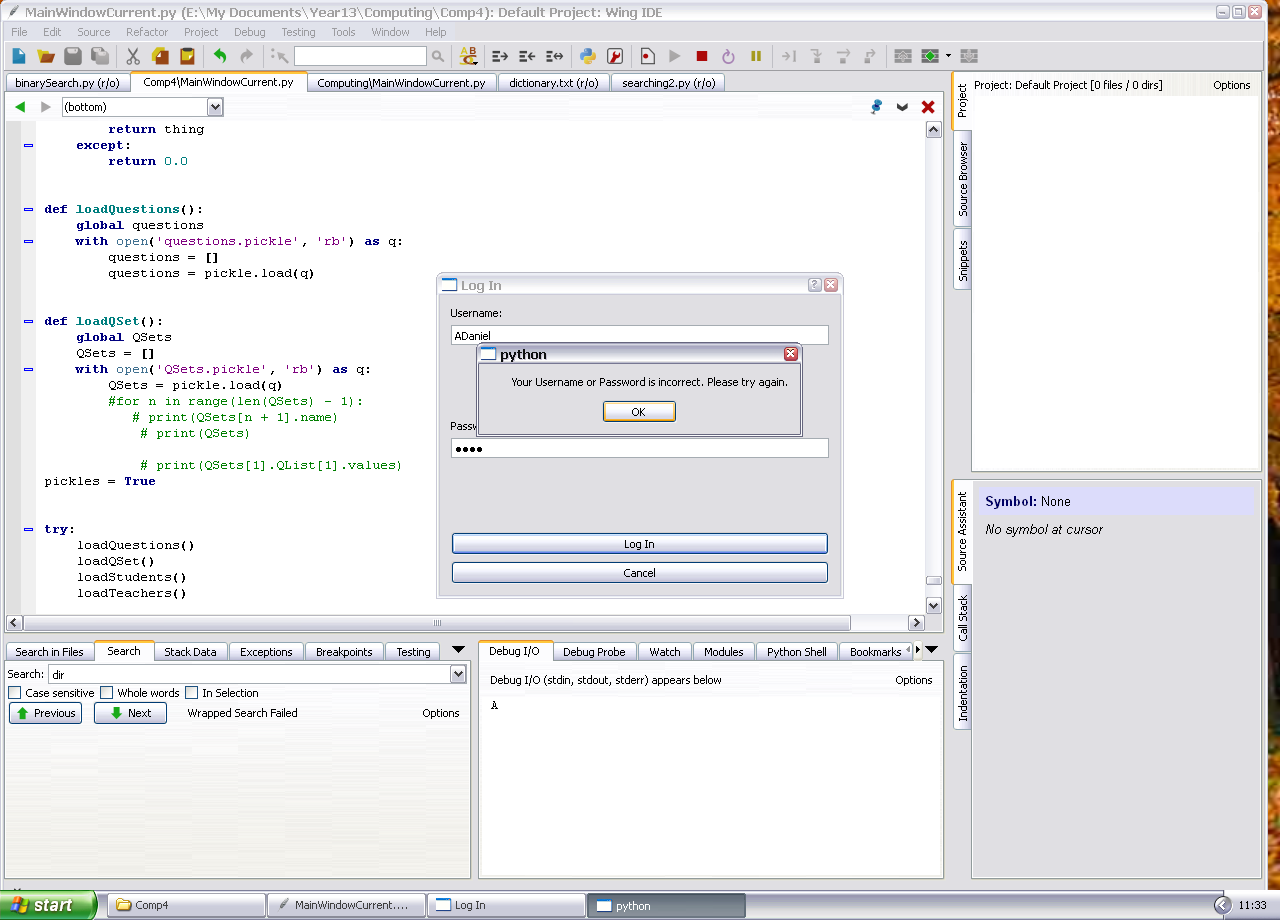
\includegraphics[width=2.0866in,height=1.6866in]{TestTable-img003.png} \\\hline
3 &
Checking that the program calculates `k' correctly. &
Typical.

(Randomly generated numbers) &
Answer being the same as on a calculator (rounded to 3sigfig). &
~

Pass &
 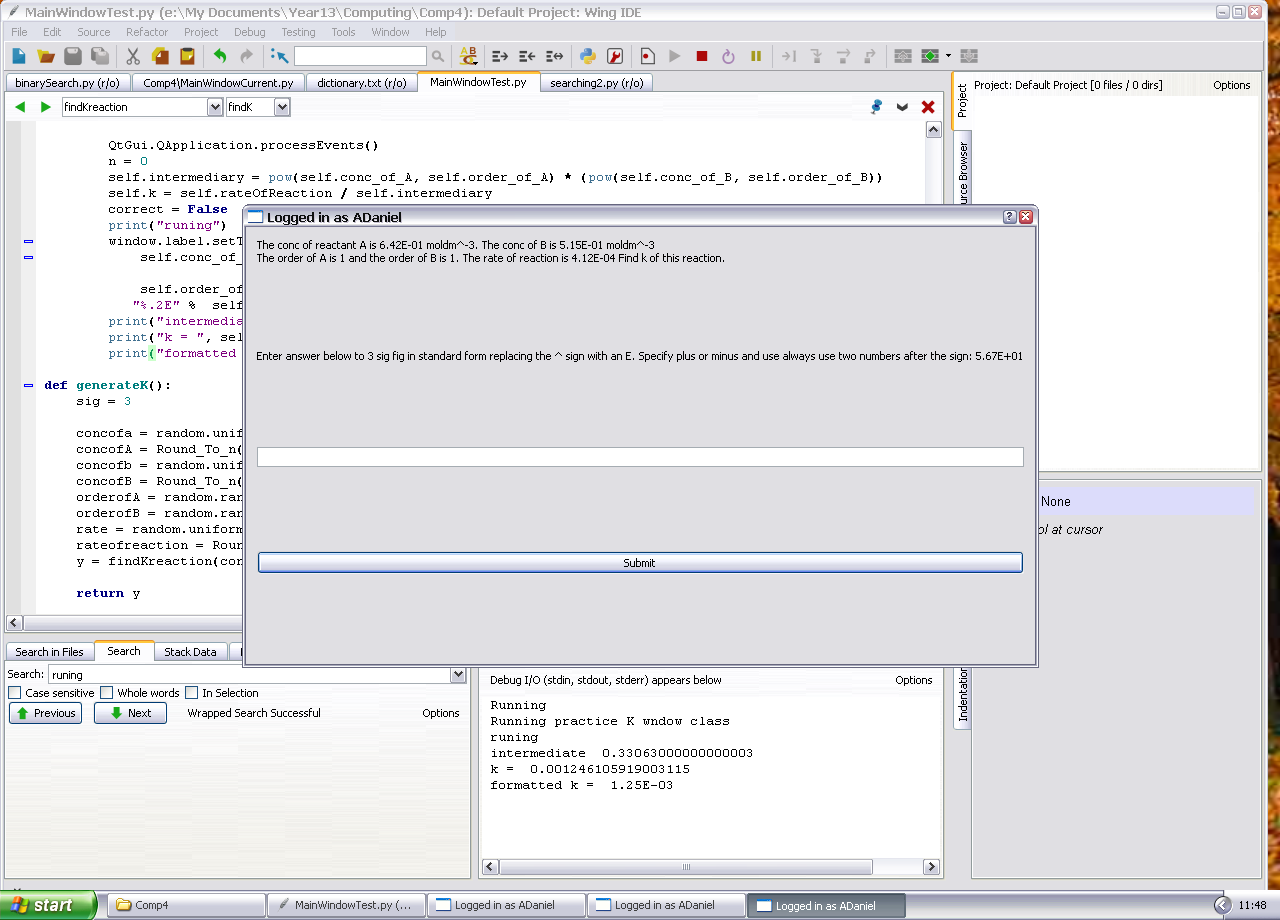
\includegraphics[width=2.3134in,height=1.7256in]{TestTable-img004.png} 
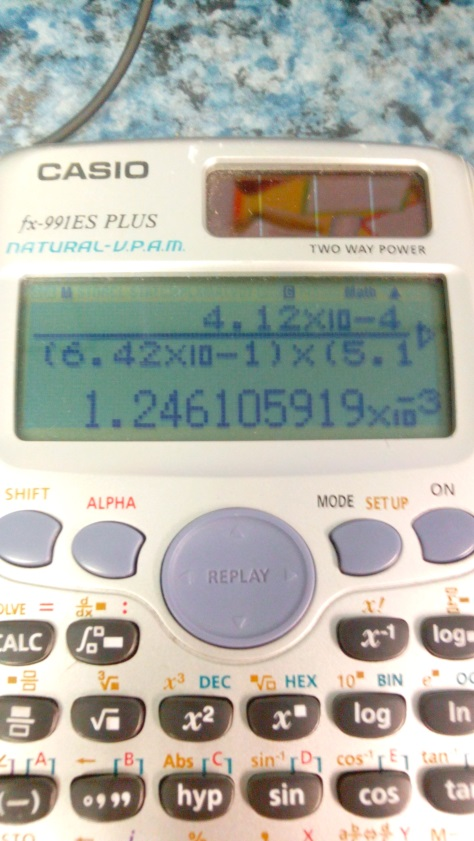
\includegraphics[width=2.1563in,height=3.8264in]{TestTable-img005.jpg} \\\hline
4 &
Checking that the program accepts correct answers for `k' values. &
Typical &
Answer calculated using correct steps, rounded to 3 sig fig and entered in the correct format. &
~

Pass &
~

~

 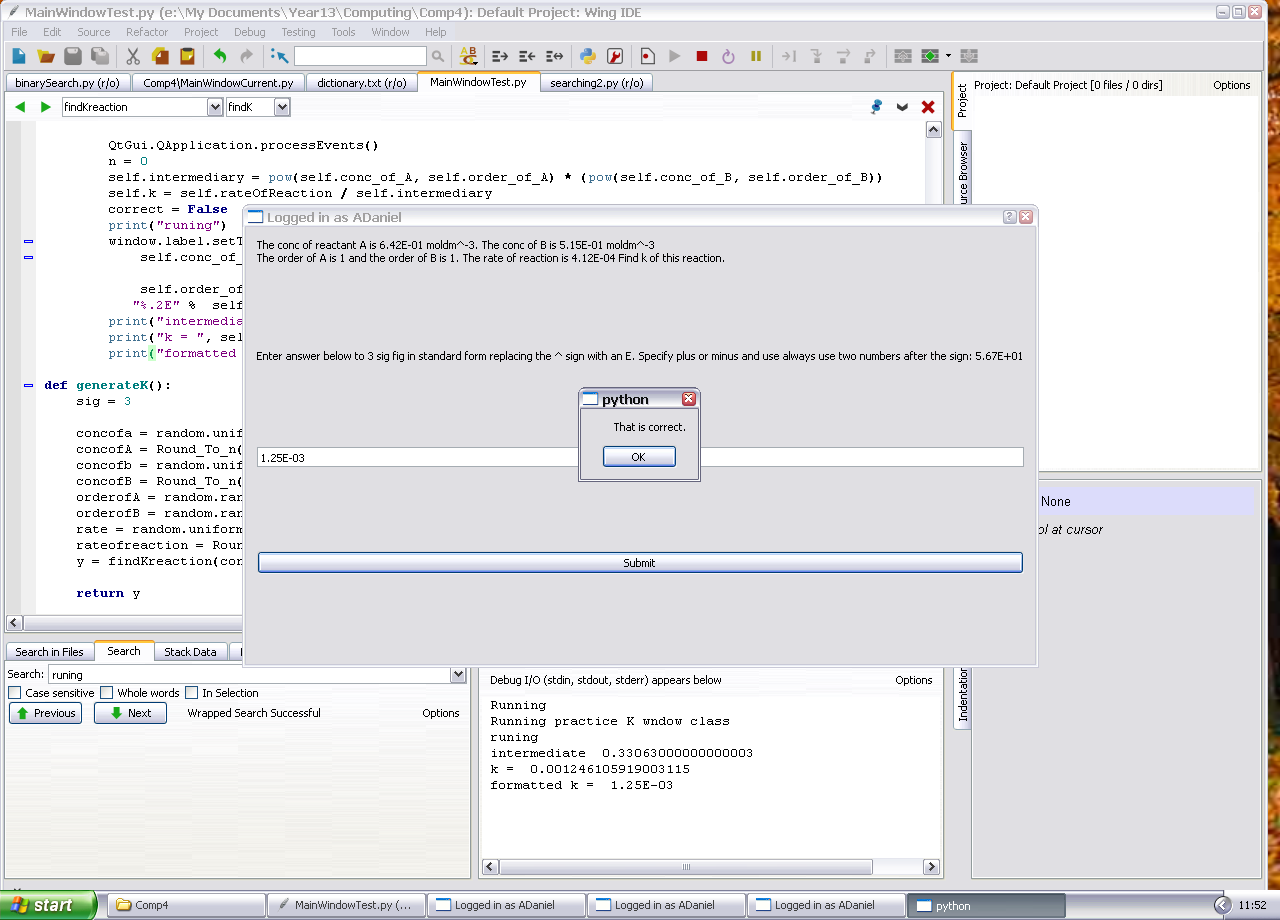
\includegraphics[width=4.0606in,height=2.3567in]{TestTable-img006.png} \\\hline
5 &
Checking that the program accepts correct answers for `k' values. &
Erroneous (any incorrect answer). &
Answer given compared to the correct answer. &
Pass &
 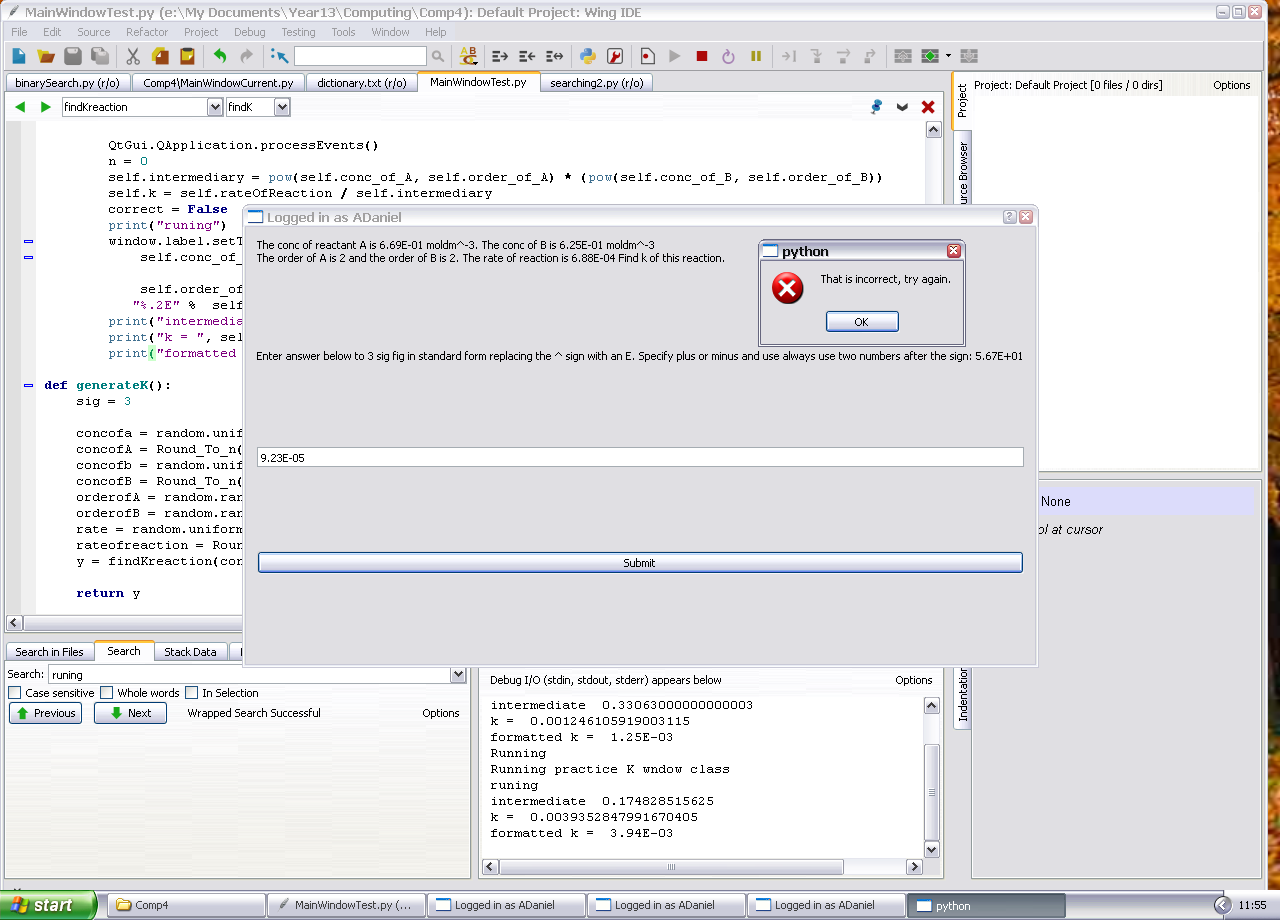
\includegraphics[angle = 90,width=1.7736in,height=1in]{TestTable-img007.png}  
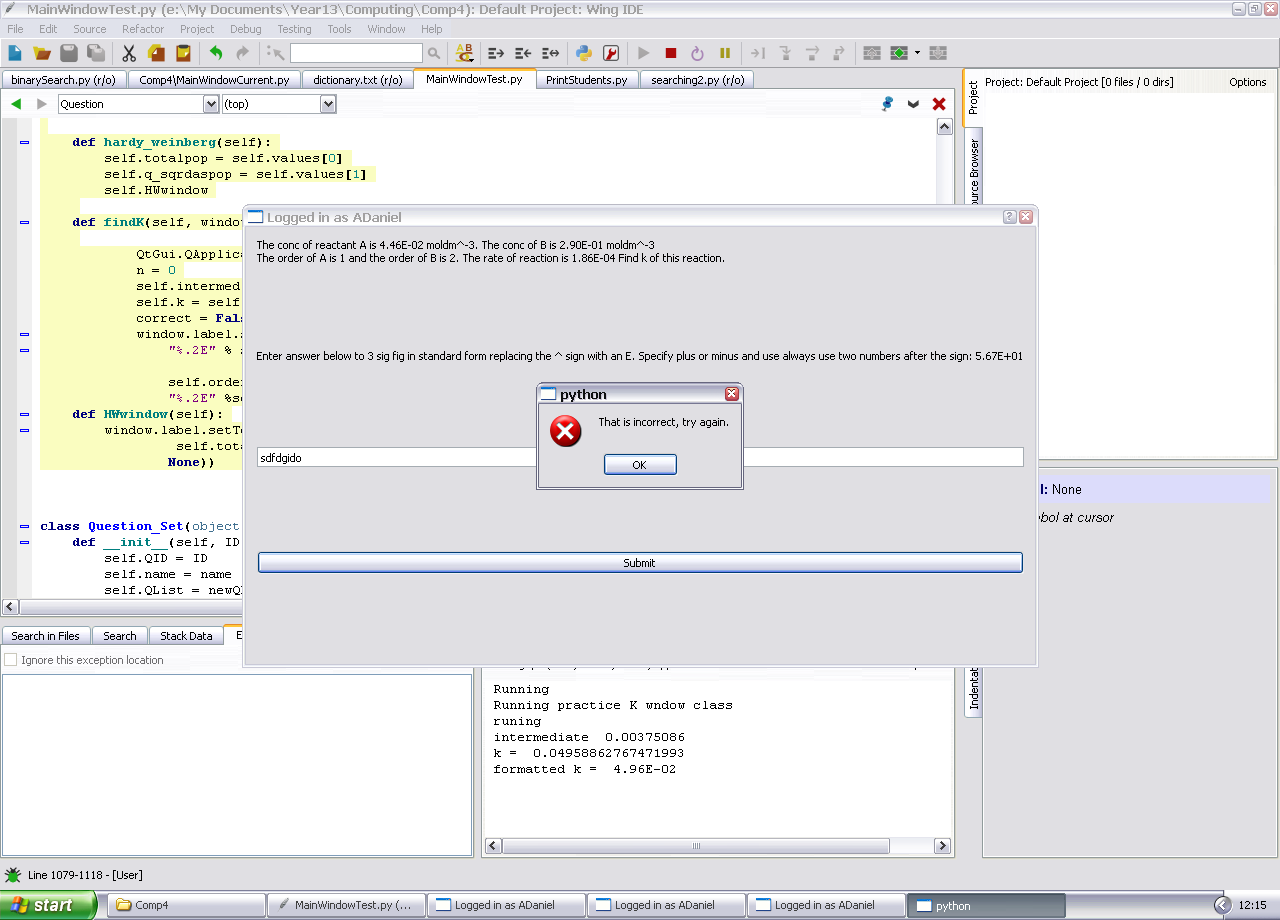
\includegraphics[angle = 90,width=3.8524in,height=1.678in]{TestTable-img008.png} 
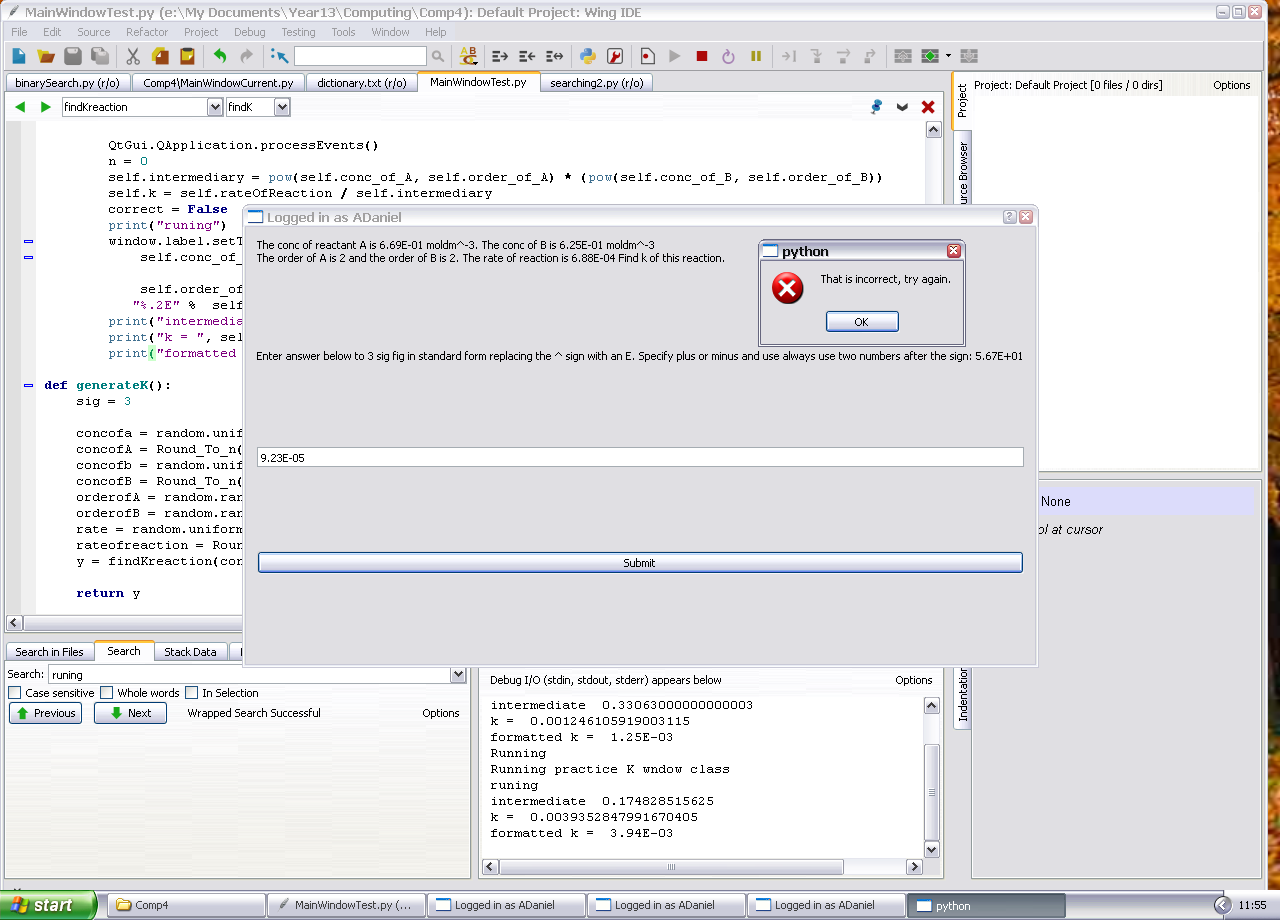
\includegraphics[angle = 90,width=3.9394in,height=2.2697in]{TestTable-img007.png} \\\hline
6 &
That an account must have a unique username, cannot have any unfilled fields apart from middle name and that a target
grade between A-U. &
Typical

(Student,Jack,William,Montfort,salmon,JMontfort, 12EJP, A) &
Student account made. &
Pass &
~

 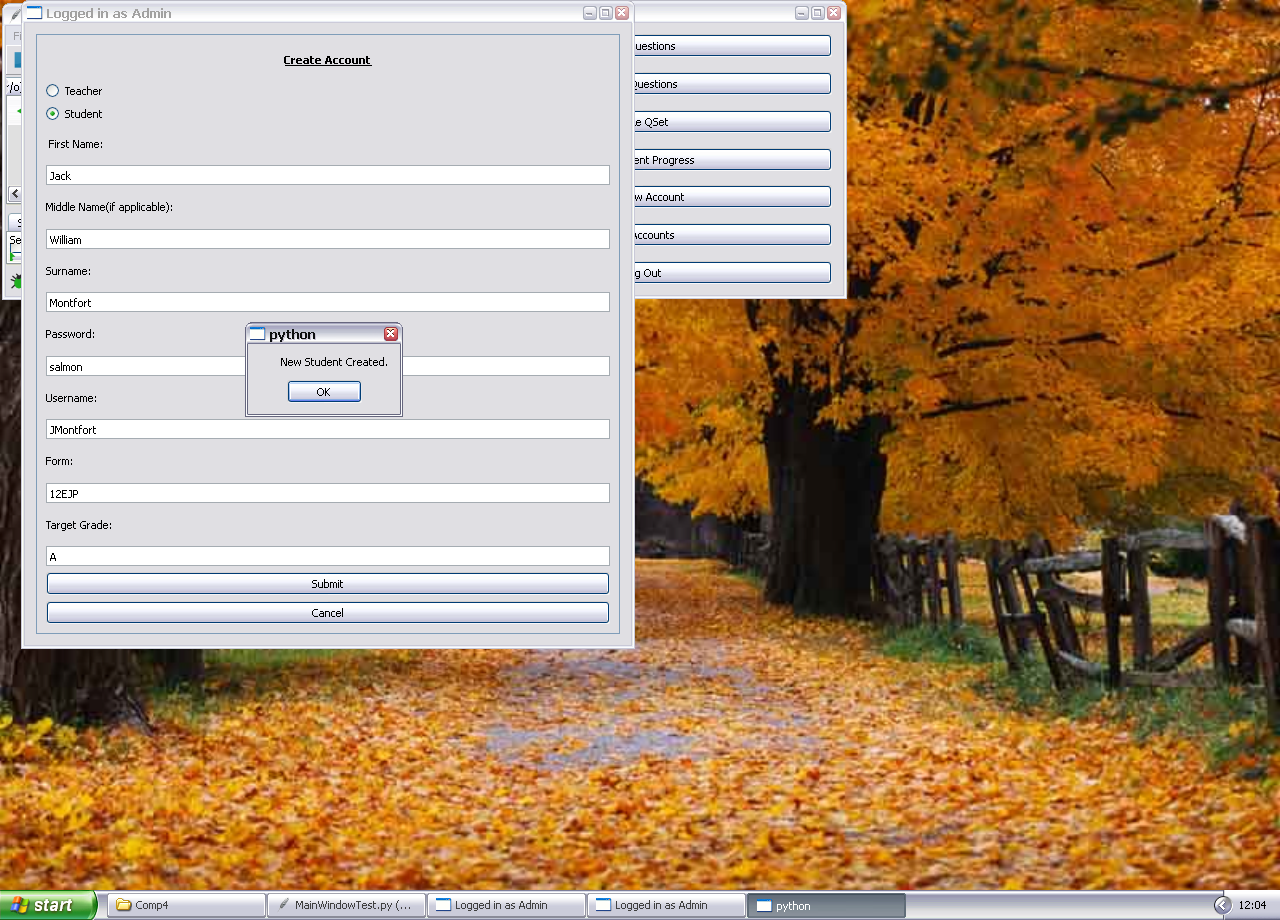
\includegraphics[width=2.278in,height=2.3819in]{TestTable-img009.png} 
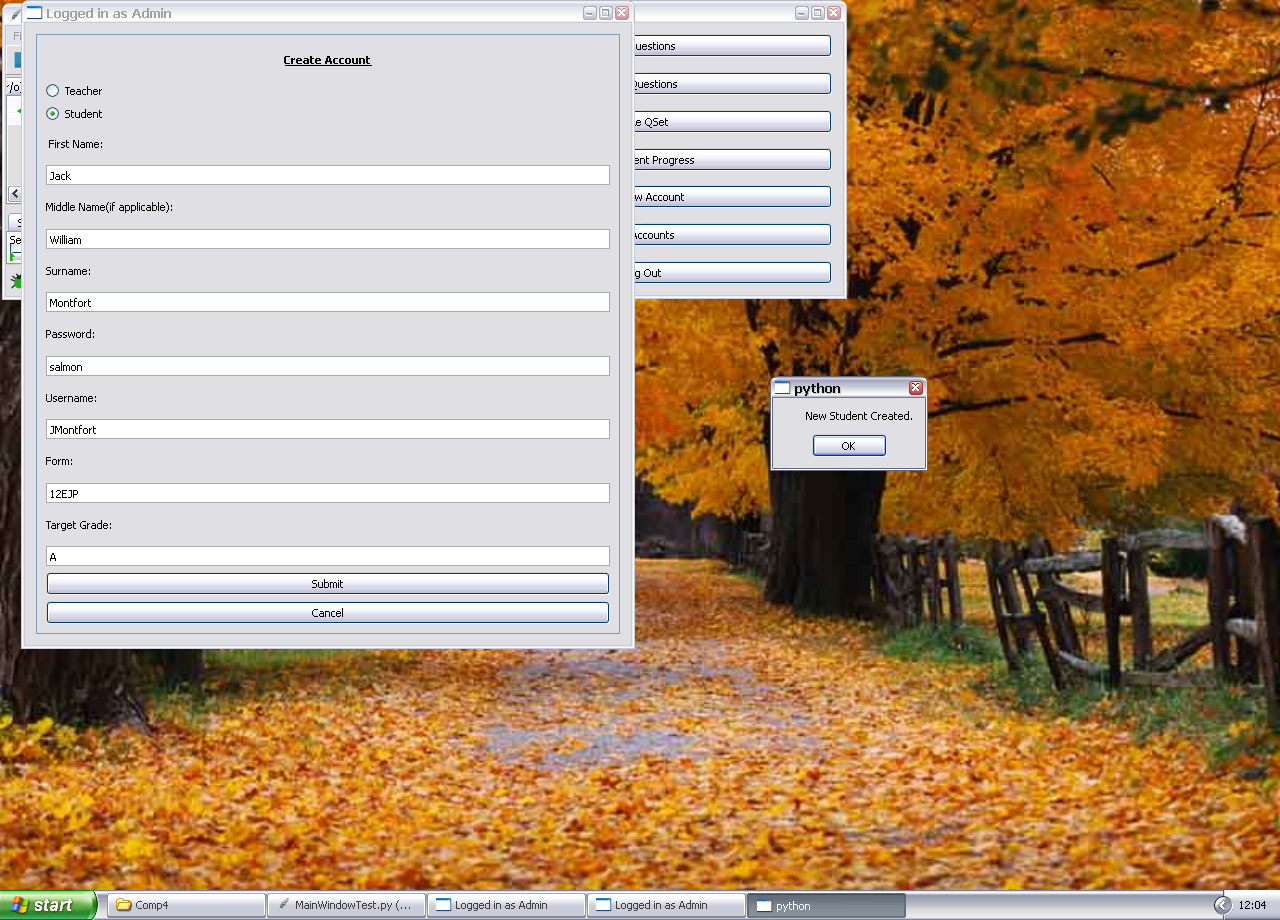
\includegraphics[width=2.2256in,height=2.3819in]{TestTable-img010.png} 
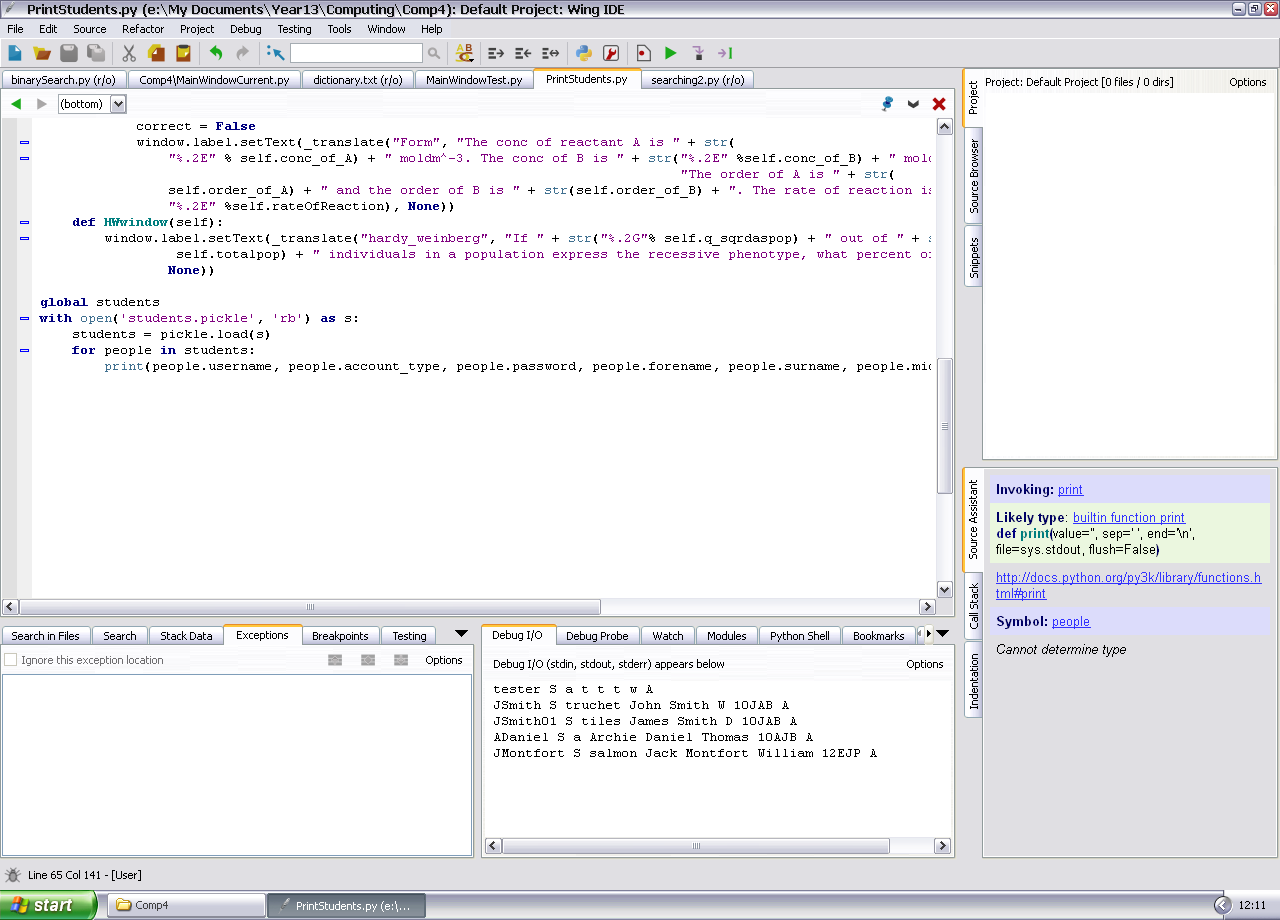
\includegraphics[width=2.3909in,height=1.2602in]{TestTable-img011.png} \\\hline
7 &
Checking that only valid information can be input into the fields. &
Erroneous

(Target grade correct as this is picked up, but the rest are not). &
Student account not made. &
Pass &
 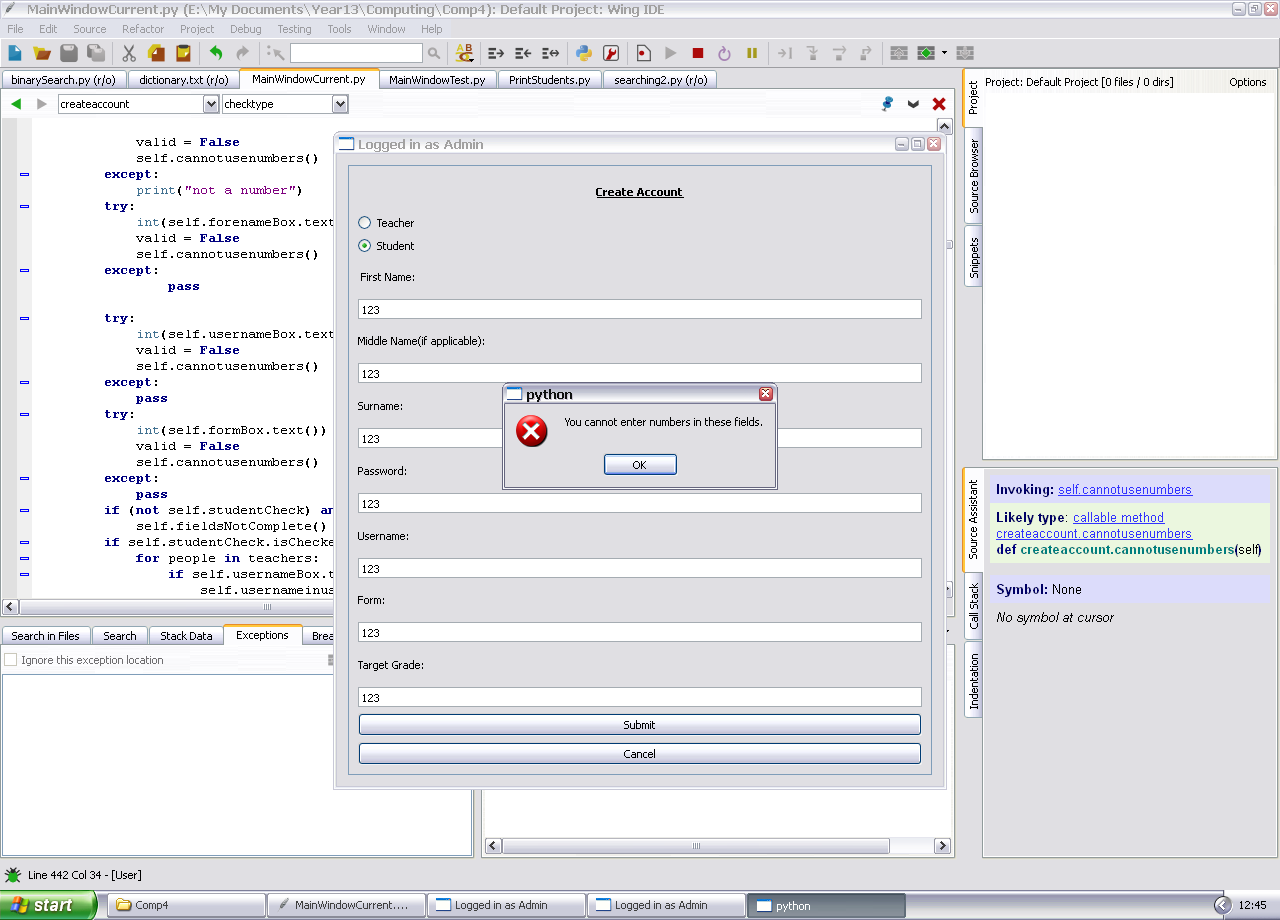
\includegraphics[width=2.9819in,height=3.1909in]{TestTable-img012.png} \\\hline
8 &
Clicking the ``Practise Questions'' button opens the ``Practise Questions'' window. &
Typical &
~
 &
~
 &
 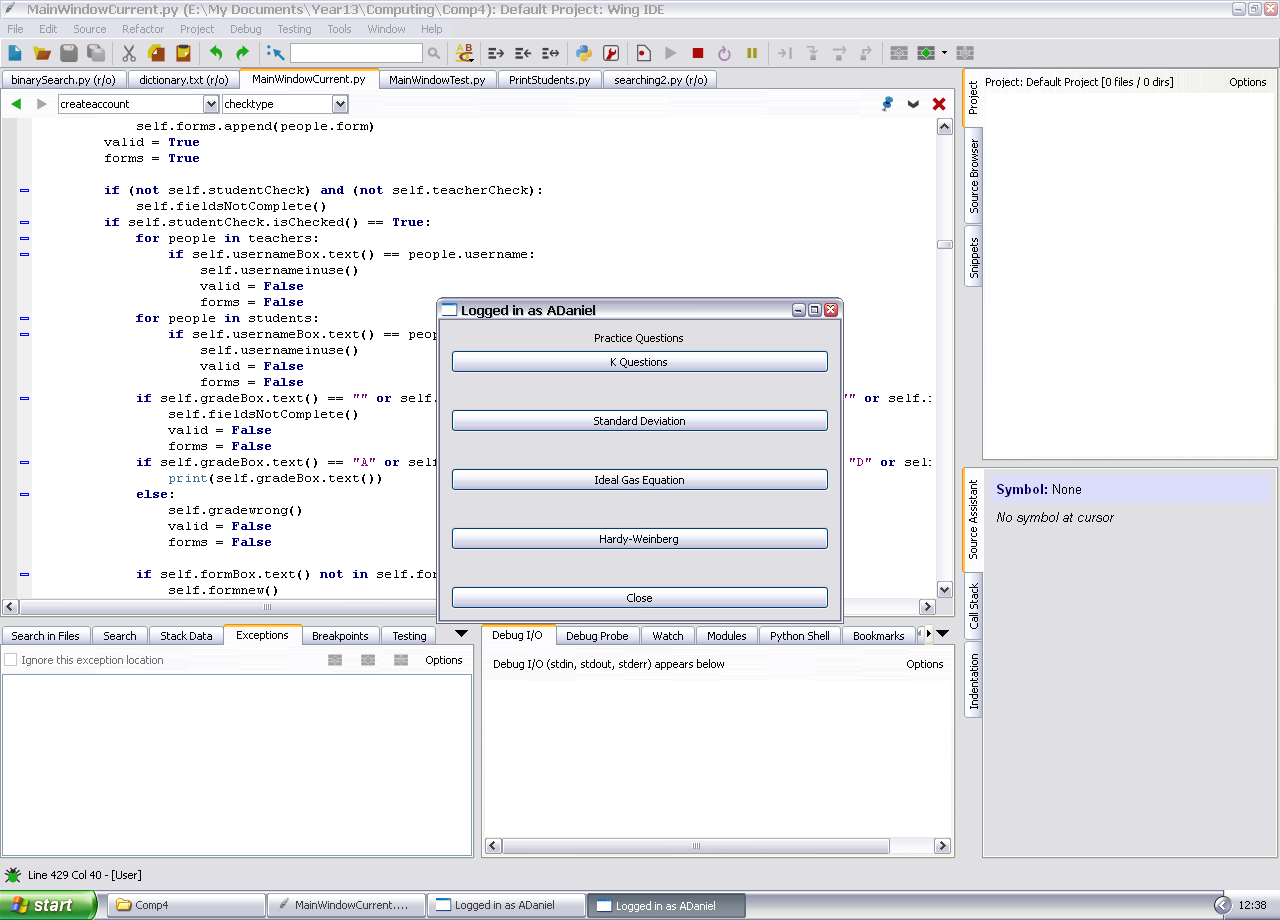
\includegraphics[width=2.0602in,height=1.6173in]{TestTable-img013.png} \\\hline
9 &
~
 &
~
 &
~
 &
~
 &
~
\\\hline
\end{supertabular}
\end{flushleft}

\bigskip


\bigskip


\bigskip


\bigskip


\bigskip


\bigskip


\bigskip


\bigskip


\bigskip


\bigskip


\bigskip


\bigskip


\bigskip
\end{document}
